\documentclass[norsk]{beamer}

%Standardpakker
\usepackage{xcolor}
\usepackage[utf8]{inputenx} % For æ, ø, å
\usepackage{babel}          % For oversettelser
\usepackage{microtype}      % Bedre typesetting
\usepackage{amssymb}        
\usepackage{mathtools}
\usepackage{xfrac}
\usepackage{graphicx}
\graphicspath{{../writeup/Figures/}}

%Spesielle pakker
\usepackage{lipsum}
\usepackage{mwe}
\usepackage{tcolorbox}

%Tikz
\usepackage{tikz}
\usetikzlibrary{quantikz}
\usetikzlibrary{graphs}

\usetheme{NSM}

\author{Thomas Wilskow Thorbjørnsen}
\title{Kvantevandringer}
\subtitle{over endelige grafer}

%%%%%%%%%%%%%%%%%%%%%%%%%%%%%%%%%%%%%%%%%%%%%%%%%%%%%%%%%%%%%%%%%

\begin{document}

\section{Introduksjon}

	\begin{frame}{Introduksjon}
		\tableofcontents
	\end{frame}

\section{Kvantemekanikk og kvanteberegninger}

	\begin{frame}{Relevant kvante}

		\begin{onlyenv}<1>
			\begin{itemize}
				\item Hva er en tilstand?
				\item Hva er en måling?
				\item Hvordan virker en tidsutvikling?
				\item Hva er et sammensatt system?
			\end{itemize}
		\end{onlyenv}

		\begin{onlyenv}<2>
			Hva en tilstand er:
			\begin{itemize}
				\item En tilstand er en ket $|\psi\rangle$, en vektor i et Hilbertrom $\mathcal{H}$.
				\item Normen til ketten er enhet: $|||\psi\rangle||=1$ 
			\end{itemize}

			Eksempel: Spin opp, spin ned.
			\begin{itemize}
				\item Anta at det finnes en partikkel med tilstandene spin opp og spin ned.
				\item Dette kan modelleres som en ket $|\psi\rangle\in \mathbb{C}\{opp,\ ned\} = \mathbb{C}^2$
				\item Ketten er i en superposisjon $|\psi\rangle = \psi_o|opp\rangle + \psi_n|ned\rangle$
			\end{itemize}
		\end{onlyenv}

		\begin{onlyenv}<3>
			Hva en måling er:
			\begin{itemize}
				\item Gitt en observabel fysisk egenskap $\mathcal{A}$ så finnes det en operator $A:\mathcal{H}\rightarrow\mathcal{H}$.
				\item Alle mulige målinger av $\mathcal{A}$ er egenverdiene til $A$.
				\item Sjansen for å måle en gitt egenverdi $a_n$ er gitt ved kvadratet av indreproduktet mellom tilstanden $|\psi\rangle$ og egenvektoren $|a_n\rangle$: $|\langle a_n|\psi\rangle|^2$.
				\item En måling kalles projektiv hvis operatoren $A$ er en projeksjon.
			\end{itemize}
		\end{onlyenv}

		\begin{onlyenv}<4>
			Hvordan tidsutvikling virker:
			\begin{itemize}
				\item For at målinger skal gi reelle verdier er det tilstrekkelig at operatoren $H$ i Schrödingers likning er hermitisk:
				\begin{align*}
					i\hbar\frac{d}{dt}|\psi(t)\rangle = H(t)|\psi(t)\rangle.
				\end{align*}
				\item En løsning av denne likningen medfører at operatoren $U$ er unitær.
				\begin{align*}
						|\psi(t)\rangle = U(t)|\psi(0)\rangle
				\end{align*}
				\item Konsekvensen er at alle operasjoner vi skal se på er unitære.
			\end{itemize}
		\end{onlyenv}

		\begin{onlyenv}<5>
			Sammensatte systemer:
			\begin{itemize}
				\item Gitt to systemer $\mathcal{H}_1$ og $\mathcal{H}_2$, så er det sammensatte systemet beskrevet av tensorproduktet: $\mathcal{H}_1\otimes\mathcal{H}_2$.
				\item Tilstandene i sammensatte systemer er gitt ved summen av elementære tensorer av basisen.
				\item En tilstand kalles sammenfiltret, hvis det ikke kan skrives som nøyaktig en elementær tensor.
				\item Bell tilstanden; $\mathcal{H}=\mathbb{C}^2\otimes\mathbb{C}^2$
				\begin{align*}
					\frac{1}{\sqrt{2}}(e_0\otimes e_0 + e_1\otimes e_1)
				\end{align*}
			\end{itemize}
		\end{onlyenv}
	\end{frame}

	\begin{frame}{Kvanteberegninger; I}
		\begin{itemize}
			\item Bits vs. Qubits \\
			\begin{onlyenv}<1>
				\begin{math}
					\{0,\ 1\}\ vs.\ \mathbb{C}\{0,\ 1\} = \mathbb{C}^2
				\end{math} \\
				\begin{math}
					0 \vee 1\ vs.\ q = q_0|0\rangle + q_1|1\rangle
				\end{math}
			\end{onlyenv}

			\begin{onlyenv}<2->
				\begin{math}
					\{0,\ 1\}^n\ vs.\ \mathbb{C}\{0,\ 1\}^n = {\mathbb{C}^2}^{\otimes n}
				\end{math} \\
				\begin{math}
					00 \vee 01 \vee 10 \vee 11\ vs.\ q = q_{00}|00\rangle + q_{01}|01\rangle + q_{10}|10\rangle + q_{11}|11\rangle
				\end{math}
			\end{onlyenv}

			\item Logiske kvanteporter \\
			\begin{onlyenv}<3>
				\begin{minipage}{0.25\textwidth}
					\begin{align*}
						X = \begin{pmatrix*}
							0 & 1 \\
							1 & 0
						\end{pmatrix*}
					\end{align*}
				\end{minipage}
				\begin{minipage}{0.25\textwidth}
					\begin{align*}
						& X(|0\rangle) = |1\rangle \\
						& X(|1\rangle) = |0\rangle
					\end{align*}
				\end{minipage}
			\end{onlyenv}

			\begin{onlyenv}<4>
				\begin{minipage}{0.25\textwidth}
					\begin{align*}
						Y = \begin{pmatrix*}
							0 & -i \\
							i & 0
						\end{pmatrix*}
					\end{align*}
				\end{minipage}
				\begin{minipage}{0.25\textwidth}
					\begin{align*}
						& Y(|0\rangle) = i|1\rangle \\
						& Y(|1\rangle) = -i|0\rangle
					\end{align*}
				\end{minipage}
			\end{onlyenv}

			\begin{onlyenv}<5>
				\begin{minipage}{0.25\textwidth}
					\begin{align*}
						Z = \begin{pmatrix*}
							1 & 0 \\
							0 & -1
						\end{pmatrix*}
					\end{align*}
				\end{minipage}
				\begin{minipage}{0.25\textwidth}
					\begin{align*}
						& Z(|0\rangle) = |0\rangle \\
						& Z(|1\rangle) = -|1\rangle
					\end{align*}
				\end{minipage}
			\end{onlyenv}

			\begin{onlyenv}<6>
				\begin{minipage}{0.3\textwidth}
					\begin{align*}
						H = \frac{1}{\sqrt{2}}\begin{pmatrix*}
							1 & 1 \\
							1 & -1
						\end{pmatrix*}
					\end{align*}					
				\end{minipage}
				\begin{minipage}{0.3\textwidth}
					\begin{align*}
						& H(|0\rangle) = \sfrac{1}{\sqrt{2}}(|0\rangle + |1\rangle) \\
						& H(|1\rangle) = \sfrac{1}{\sqrt{2}}(|0\rangle - |1\rangle)
					\end{align*}
				\end{minipage}
			\end{onlyenv}

			\begin{onlyenv}<7>
				\begin{minipage}{0.35\textwidth}
					\begin{align*}
						CNOT = \begin{pmatrix*}
							1 & 0 & 0 & 0 \\
							0 & 1 & 0 & 0 \\
							0 & 0 & 0 & 1 \\
							0 & 0 & 1 & 0
						\end{pmatrix*}
					\end{align*}
				\end{minipage}
				\begin{minipage}{0.35\textwidth}
					\begin{align*}
						& CNOT(|00\rangle) = |00\rangle \\
						& CNOT(|01\rangle) = |01\rangle \\
						& CNOT(|10\rangle) = |11\rangle \\
						& CNOT(|11\rangle) = |10\rangle
					\end{align*}
				\end{minipage}
			\end{onlyenv}

		\end{itemize}
	\end{frame}

	\begin{frame}{Kvanteberegninger; II}
		\begin{itemize}
			\item Bell state
			\begin{flushleft}
				\begin{minipage}{0.35\textwidth}
					\begin{quantikz}
						\lstick{$\ket{0}$} & \gate{H} & \octrl{1} & \qw \\
						\lstick{$\ket{0}$} & \qw & \targ{} & \qw
					\end{quantikz}
				\end{minipage}
				\begin{minipage}{0.35\textwidth}
					\begin{math}
						\iff CNOT\circ (H\otimes I) 
					\end{math}
				\end{minipage}
			\end{flushleft}
			\begin{onlyenv}<2->
				\item Universelle porter
			\end{onlyenv}
			
			\begin{onlyenv}<3->
				\item Simulere klassiske beregninger
			\end{onlyenv}
			
			\begin{onlyenv}<3>
				\begin{quantikz}
					\lstick[wires=3]{$\psi$} & \octrl{1} & \qw & \qw \rstick[wires=3]{Toffoli} \\
					& \octrl{1} & \qw & \qw \\
					& \targ{} & \qw & \qw
				\end{quantikz}
			\end{onlyenv}
			
			\begin{onlyenv}<4>
				\begin{quantikz}
					\lstick[wires = 2]{$\psi$} & \octrl{1} & \qw \rstick[wires = 2]{$\psi$} & \rstick[wires = 3]{AND} \\
					& \octrl{1} & \qw \\
					\lstick{$\ket{0}$} & \targ{} & \qw & \qw
				\end{quantikz}
			\end{onlyenv}

			\begin{onlyenv}<5>
				\begin{quantikz}
					\lstick{$\ket{1}$} & \octrl{1} & \qw \rstick{$\ket{1}$} & \rstick[wires = 3]{NOT} \\
					\lstick{$\ket{1}$} & \octrl{1} & \qw \rstick{$\ket{1}$} \\
					\lstick{$\psi$} & \targ{} & \qw & \qw
				\end{quantikz}
			\end{onlyenv}

			\begin{onlyenv}<6>
				\begin{quantikz}
					\lstick[wires = 2]{$\psi$} & \gate{X} & \octrl{1} & \gate{X} & \qw \rstick[wires = 2]{$\psi$} & \rstick[wires = 3]{OR} \\
					& \gate{X} & \octrl{1} & \gate{X} & \qw \\
					\lstick{$\ket{1}$} & \qw & \targ{} & \qw & \qw & \qw
				\end{quantikz}
			\end{onlyenv}
		\end{itemize}
	\end{frame}

	\begin{frame}{Kvanteberegninger; III}
		\begin{center}
			\begin{quantikz}
				\lstick{$\ket{1}$} & \octrl{1} & \octrl{1} & \qw & \octrl{1} & \octrl{1} & \qw \rstick{$\ket{1}$} & \rstick[wires = 5]{OR} \\
				\lstick{$\ket{1}$} & \octrl{1} & \octrl{2} & \qw & \octrl{1} & \octrl{2} & \qw \rstick{$\ket{1}$} \\
				\lstick[wires = 2]{$\psi$} & \targ{} & \qw & \octrl{1} & \targ{} & \qw & \qw \rstick[wires = 2]{$\psi$} \\
				& \qw & \targ{} & \octrl{1} & \qw & \targ{} & \qw \\
				\lstick{$\ket{1}$} & \qw & \qw & \targ{} & \qw & \qw & \qw & \qw
			\end{quantikz}
		\end{center}
	\end{frame}

	\begin{frame}{Orakler}
		\begin{itemize}
			\item Algoritmer trenger å spørre på en eller annen måte
			
			\begin{onlyenv}<1>
				\item Kvanteparallellisme
				\item Merkeorakler
				\begin{align*}
					f & : \{0,\ 1\}^n\rightarrow \{0,\ 1\} \\
					\mathcal{O}_f & : \mathbb{C}\{0,\ 1\}^n \otimes \mathbb{C}\{0,\ 1\} \rightarrow \mathbb{C}\{0,\ 1\}^n \otimes \mathbb{C}\{0,\ 1\} \\
					& |x\rangle|y\rangle \mapsto |x\rangle|y\oplus f(x)\rangle
				\end{align*}
			\end{onlyenv}

			\begin{onlyenv}<2>
				\item Kvanteparallellisme
				\item Faseorakler
				\begin{align*}
					f & : \{0,\ 1\}^n\rightarrow \{0,\ 1\} \\
					\mathcal{O}_{f,\pm} & : \mathbb{C}\{0,\ 1\}^n \rightarrow \mathbb{C}\{0,\ 1\}^n \\
					& |x\rangle \mapsto (-1)^{f(x)}|x\rangle
				\end{align*}
			\end{onlyenv}

			\begin{onlyenv}<3>
				\item Transformere merkeorakel til faseorakel \\
				\begin{quantikz}
                    \lstick{$\ket{z}$} & \qw\gategroup[wires=2, steps=9, style={dashed, rounded corners, fill=blue!5, inner xsep=2pt}, background]{$O_{f,\pm}$} & \qw & \qw & \qw & \gate[2]{O_f} & \qw & \qw & \qw & \qw & \qw \rstick{$(-1)^{f(z)}\ket{z}$}\\
                    & & \lstick{$\ket{0}$} & \gate{X} & \gate{H} & & \gate{H} & \gate{X} & \qw \rstick{$\ket{0}$} &
                \end{quantikz}
			\end{onlyenv}
		\end{itemize}
	\end{frame}

	\begin{frame}{Deutsch-Jozsa}
		\begin{itemize}
			\item Problemet:
			\begin{itemize}
				\item La $f : \{0,\ 1\}^n \rightarrow \{0,\ 1\}$ være en funksjon som enten er konstant eller balansert ($50\%$ er $0$ og $50\%$ er $1$).
			\end{itemize}
			\item Mål: Finne ut om $f$ er konstant eller balansert.
			
			\begin{onlyenv}<2>
				\item Klassisk løsning:
				\begin{enumerate}
					\item Evaluere $f$ i $\frac{2^n}{2}+1$ elementer.
					\item Hvis alle er $0$ eller $1$ fastslå konstant, hvis ikke fastslå balansert.
				\end{enumerate}
			\end{onlyenv}
			
			\begin{onlyenv}<3>
				\item Kvante løsning:
				\begin{center}
					\begin{quantikz}
						\lstick[wires = 3]{$|0\rangle^{\otimes n}$} & \gate{H} & \gate[3]{O_{f,\pm}} & \gate{H} & \qw \\
						& \gate{H} & & \gate{H} & \qw \\
						& \gate{H} & & \gate{H} & \qw
					\end{quantikz}
				\end{center}
			\end{onlyenv}
		\end{itemize}
	\end{frame}

\section{Grover's algoritme og Amplitudeforsterkningsteknikken}

	\begin{frame}{Grover's algoritme; I}
		\begin{itemize}
			\item Problemet:
				\begin{itemize}
					\item La $f : \{0,\ 1\}^n \rightarrow \{0,\ 1\}$ være en funksjon
				\end{itemize}

			\item Mål: Finne et element som evalueres til $1$.

			\begin{onlyenv}<2>
				\item Klassisk løsning: 
				\begin{enumerate}
					\item Evaluer hvert element fra $0$ til $2^n-1$.
					\item Stopp når man finner et element $z$ slik at $f(z) = 1$.
				\end{enumerate}
			\end{onlyenv}
				
			\begin{onlyenv}<3>
				\item Kvante løsning:
				\begin{quantikz}
					\lstick[wires = 3]{$|0\rangle^{\otimes n}$} & \gate{H} & \gate[3]{O_{f,\pm}}\gategroup[wires = 3, steps = 4, style = {rounded corners}]{G} & \gate{H} & \gate[wires = 3]{R} & \gate{H} & \gate[3]{G} & \qw \ldots & \gate[3]{G} & \qw \\
					& \gate{H} & & \gate{H} & & \gate{H} & & \qw \ldots & & \qw \\
					& \gate{H} & & \gate{H} & & \gate{H} & & \qw \ldots & & \qw
				\end{quantikz}
			\end{onlyenv}
		\end{itemize}
	\end{frame}

	\begin{frame}{Grover's algoritme; II}
		\begin{itemize}
			\item Hva er R?
			\begin{align*}
				R = \begin{pmatrix*}
					1 & 0 & 0 & ... \\
					0 & -1 & 0 & ... \\
					0 & 0 & -1 & ... \\
					\vdots & \vdots & \vdots & \ddots
				\end{pmatrix*} = 2|0\rangle^{\otimes n}\langle 0|^{\otimes n} - I
			\end{align*}
			\item Hva er H$^{\otimes n}$RH$^{\otimes n}$?
			\begin{align*}
				H^{\otimes n}RH^{\otimes n} = 2(H|0\rangle\langle 0|H)^{\otimes n}-I = 2dd^*-I \\
				d = \frac{1}{\sqrt{2}^n}\Sigma_{z=0}^{2^n}|z\rangle
			\end{align*}
		\end{itemize}		
	\end{frame}

	\begin{frame}{Grover's algoritme, III}
		\begin{itemize}
			\item Definer to tilstander
			\begin{align*}
				g & = \frac{1}{\sqrt{t}}\sum_{f(z)=1}|z\rangle \\
				b & = \frac{1}{\sqrt{2^n-t}}\sum_{f(z) = 0}|z\rangle
			\end{align*}
			\begin{minipage}{0.3\textwidth}
				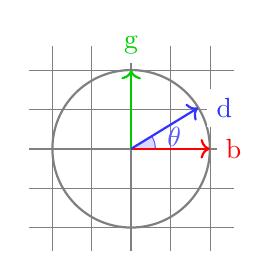
\begin{tikzpicture}
					\draw[step=.5,gray,very thin] (-1.3,-1.3) grid (1.3,1.3);
					\draw[gray, thick] (0,0) circle (1);
					\draw[gray, thick] (1.3, 0) -- (-1.3, 0);
					\draw[gray, thick] (0, 1.3) -- (0, -1.3);
					\draw[green!80!black, thick, ->] (0,0) -- (0, 1) node[above=2pt, fill=white] {g};
					\draw[blue!65!white, thick] (0.3, 0) arc (0:30:0.3) node[right=2pt] {$\theta$};
					\fill[blue!15!white] (0,0) -- (0.3, 0) arc (0:30:0.3) -- (0,0);
					\draw[red, thick, ->] (0,0) -- (1,0) node[right=2pt, fill=white] {b};
					\draw[blue!80!white, thick, ->] (0,0) -- (0.85,0.52) node[right=3pt, fill=white] {d};
				\end{tikzpicture}
			\end{minipage}
			\begin{minipage}{0.35\textwidth}
				\item Velg $\theta$
				\begin{align*}
					\theta & = \arcsin(\frac{\sqrt{t}}{\sqrt{2}^n}) \\
					d & = \sin(\theta)g + \cos(\theta)b
				\end{align*}
			\end{minipage}
		\end{itemize}
	\end{frame}

	\begin{frame}{Grover's algoritme; IV}
		\begin{itemize}
			\item $\mathcal{O}_{f,\pm}$ er en refleksjon i planet $\mathbb{C}\{g,\ b\}$.
			\begin{align*}
				& \mathcal{O}_{f,\pm}(g) = -g \\
				& \mathcal{O}_{f,\pm}(b) = b
			\end{align*}
			\begin{center}				
				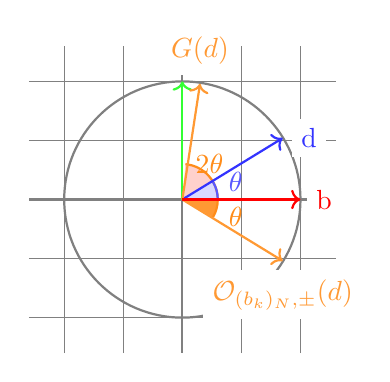
\begin{tikzpicture}[scale=1.5]
					\draw[step=.5,gray,very thin] (-1.3,-1.3) grid (1.3,1.3);
					\draw[gray, thick] (0,0) circle (1);
					\draw[gray, thick] (1.3, 0) -- (-1.3, 0);
					\draw[gray, thick] (0, 1.3) -- (0, -1.3);
					\draw[green!80!white, thick, ->] (0,0) -- (0, 1) node[above=2pt, fill=white] {g};
					\fill[red!80!orange!20!white] (0,0) -- (0.3, 0) arc (0:85:0.3) -- (0,0);
					\fill[blue!15!white] (0,0) -- (0.3, 0) arc (0:30:0.3) -- (0,0);
					\fill[orange!80!white] (0,0) -- (0.3, 0) arc (0:-30:0.3) -- (0,0);
					\draw[orange!90!white, thick] (0.3, 0) arc (0:85:0.3) node[right=0pt] {$2\theta$};
					\draw[blue!65!white, thick] (0.3, 0) arc (0:30:0.3) node[right=2pt] {$\theta$};
					\draw[orange!90!white, thick] (0.3, 0) arc (0:-30:0.3) node[right=2pt] {$\theta$};
					\draw[blue!80!white, thick, ->] (0,0) -- (0.85,0.52) node[right=3pt, fill=white] {d};
					\draw[orange!80!white, thick, ->] (0,0) -- (0.15,0.98) node[above=3.2pt, fill=white] {$G(d)$};
					\draw[orange!80!white, thick, ->] (0,0) -- (0.85,-0.52) node[below=3pt, fill=white] {$\mathcal{O}_{(b_k)_N,\pm}(d)$};
					\draw[red, thick, ->] (0,0) -- (1,0) node[right=2pt, fill=white] {b};
				\end{tikzpicture}
			\end{center}
		\end{itemize}
	\end{frame}

	\begin{frame}{Grover's algoritme; V}
		\begin{itemize}
			\item Kjøretidsanalyse
			\begin{align*}
				G(d) & = \sin(3\theta)g + \cos(3\theta)b \\
				\implies G^k(d) & = \sin((2k+1)\theta)g + \cos((2k+1)\theta)b
			\end{align*}
			\begin{itemize}
				\begin{onlyenv}<1>
					\item Maksima når $\sin((2k+1)\theta)=1$
					\begin{align*}
						k & = \frac{\pi}{4\theta} - \frac{1}{2} \approx \lfloor\frac{\pi}{4\arcsin(\sfrac{\sqrt{t}}{\sqrt{N}})}\rfloor \\
						p & = \sin((1+2\lfloor\frac{\pi}{4\arcsin(\sfrac{\sqrt{t}}{\sqrt{N}})}\rfloor)\arcsin(\sfrac{\sqrt{t}}{\sqrt{N}}))
					\end{align*}
				\end{onlyenv}

				\begin{onlyenv}<2>
					\item $\sin(\sfrac{\sqrt{t}}{\sqrt{N}}) \approx \sfrac{\sqrt{t}}{\sqrt{N}}$ når $N \gg 1$.
					\begin{align*}
						k & = \lfloor\frac{\pi\sqrt{N}}{4\sqrt{t}}\rfloor \\
						p & = \sin((1 + 2\lfloor\frac{\pi\sqrt{N}}{4\sqrt{t}}\rfloor)\frac{\sqrt{t}}{\sqrt{N}})
					\end{align*}
				\end{onlyenv}
			\end{itemize}
		\end{itemize}
	\end{frame}

	\begin{frame}{Amplitudeforsterkningsteknikken}
		\begin{itemize}
			\begin{onlyenv}<1-2>
				\item Sannsynlighetforsterkning
				\begin{itemize}
					\item Anta at $A$ er en klassisk Monte Carlo algoritme
					\item Anta at vi kan sjekke om en løsning er korrekt i polynom tid
					\item La $\psi_0$ være inputet og $\psi = A(\psi_0)$ være et output
					\item Anta at $p$ er sannsynligheten for at $\psi$ er et korrekt svar
					\item Hvordan kan vi forbedre algoritmen og øke sjansen for at $A$ gir oss riktig svar?
					\begin{onlyenv}<2>
						\item Vi kjører $A$ flere ganger, si $n$ ganger.
						\item Hvis $p\ll 1$ så gir $n = \sfrac{1}{p}$ et godt estimat for maksima.
					\end{onlyenv}	
				\end{itemize}
			\end{onlyenv}

			\begin{onlyenv}<3>
				\item Anta at $A$ er en kvantealgoritme
				\item La $\psi_0$ være inputet og $\psi = A(\psi_0)$ være et output
				\item Anta at det finnes et faseorakel $\mathcal{O}_{\pm}$ som sjekker om outputet er korrekt
				\item Anta at $p$ er sannsynligheten for at $\psi$ er et korrekt svar
				\item Hvordan kan vi forbedre algoritmen og øke sjansen for at $A$ gir oss riktig svar?
			\end{onlyenv}

			\begin{onlyenv}<4->
				\item Algoritme $A$, input $\psi_0$, output $\psi$, faseorakel $\mathcal{O}_{\pm}$ og $p$
				\item Hvordan kan vi forbedre algoritmen og øke sjansen for at $A$ gir oss riktig svar?
			\end{onlyenv}

			\begin{onlyenv}<5>
				\begin{align*}
					U' = 2|\psi\rangle\langle \psi| - I
				\end{align*}
				\begin{center}
					\begin{quantikz}
						\lstick{$\psi_0$} & \gate{A} & \gate{O_\pm}\gategroup[wires = 1, steps = 2, style = {rounded corners}]{U} & \gate{U'} & \gate{U} & \qw\ldots & \gate{U} & \qw
					\end{quantikz}
				\end{center}
			\end{onlyenv}

			\begin{onlyenv}<6>
				% \item Analyse \\
				\begin{minipage}{0.45\textwidth}
					\begin{align*}
						\psi & = \sum_{z:\{0,\ 1\}^n}\zeta_z|z\rangle \\
						g & = \frac{1}{\sqrt{p}}\sum_{f(z)=1}\zeta_z|z\rangle \\
						b & = \frac{1}{\sqrt{1-p}}\sum_{f(z)=0}\zeta_z|z\rangle
					\end{align*}
				\end{minipage}%
				\begin{minipage}{0.45\textwidth}
					\begin{align*}
						\theta & = \arcsin(\sqrt{p}) \\
						k & = \lfloor\frac{\pi}{4\arcsin(\sqrt{p})}\rfloor \approx \lfloor\frac{\pi}{4\sqrt{p}}\rfloor \\
						p' & \approx \sin^2(\frac{\pi}{2}+\sqrt{p})
					\end{align*}
				\end{minipage}
			\end{onlyenv}
		\end{itemize}
		
	\end{frame}

\section{Kvantevandringer}

	\begin{frame}{Kvantevandringer}
		\begin{itemize}
			\item Generalisering av Grover's algoritme
			\item Hva er en graf? $G=(V,E)$; $\mathcal{H} = \mathbb{C}V$
			\item Lokale operatorer
			\item Komponenter til andre algoritmer
			\item Myntede vandringer
			\begin{itemize}
				\item Position-coin notation
				\item Arc notation
			\end{itemize}
			\item Umyntede vandringer
			\item QSS
		\end{itemize}
	\end{frame}

	\begin{frame}{Position-coin notation}
		\begin{itemize}
			\item $d$-regulær, $d$-kantkromatisk graf
			\item Fra enhver node, velger vi en farge og følger den
			\item $\mathcal{H} = \mathbb{C}V \otimes \mathbb{C}^d$
			
			\begin{onlyenv}<1>
				\begin{minipage}{0.35\textwidth}
					\begin{center}
						\begin{quantikz}
							\lstick{$\mathbb{C}V$} & \qw\gategroup[wires = 2, steps = 2, style={rounded corners}]{U} & \gate[2]{S} & \qw \\
							\lstick{$\mathbb{C}^d$} & \gate{C} & & \qw
						\end{quantikz}
					\end{center}
				\end{minipage}%
				\begin{minipage}{0.5\textwidth}
					\begin{center}
						
						\item $S$ er flip-flop operatoren
						\begin{align*}
							S^2 = I
						\end{align*}
						\item $C$ er coin operatoren
					\end{center}
				\end{minipage}
			\end{onlyenv}


			\begin{onlyenv}<2>
				\begin{minipage}{0.35\textwidth}
					\begin{center}
						\item S er definert av fargeleggingen
						\item Vi kan velge C
						\begin{align*}
							C = H\otimes H
						\end{align*}
					\end{center}
				\end{minipage}%
				\begin{minipage}{0.4\textwidth}
					
					\begin{center}
						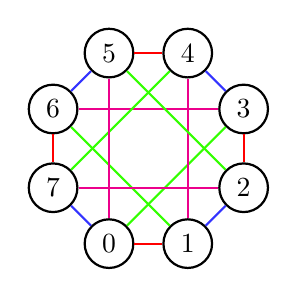
\begin{tikzpicture}[thick, main/.style = {draw, circle}]
							\node[main] (1) at (0,0) {0};
							\node[main] (2) at (1,0) {1};
							\node[main] (3) at (1.71, 0.71) {2};
							\node[main] (4) at (1.71, 1.71) {3};
							\node[main] (5) at (1, 2.42) {4};
							\node[main] (6) at (0, 2.42) {5};
							\node[main] (7) at (-0.71, 1.71) {6};
							\node[main] (8) at (-0.71, 0.71) {7};
							\graph {
								(1) --[color=red] (2) --[color=blue!80!white] (3) --[color=red] (4) --[color=blue!80!white] (5) --[color=red] (6) --[color=blue!80!white] (7) --[color=red] (8) --[color=blue!80!white] (1) --[color=green!80!yellow] (4) --[color=magenta] (7) --[color=green!80!yellow] (2) --[color=magenta] (5) --[color=green!80!yellow] (8) --[color=magenta] (3) --[color=green!80!yellow] (6) --[color=magenta] (1);
								};
							\end{tikzpicture}
						\end{center}
					\end{minipage}
				\end{onlyenv}
			\end{itemize}
	\end{frame}

	\begin{frame}{Arc notation}
		\begin{itemize}
			\item Virker på generelle grafer
			\item Kan tolkes som en vandring på kantene istedenfor nodene
			\item $\mathcal{H} = \bigoplus_{v:V}\mathbb{C}\{u:V\mid (v,u):E\} \simeq \bigoplus_{v:V}\mathbb{C}^{deg(v)}$
			\item $\mathcal{H} \subseteq \mathbb{C}V \otimes \mathbb{C}V$
			
			\begin{onlyenv}<1-2>
				\begin{minipage}{0.35\textwidth}
					\begin{quantikz}
						\lstick{$\mathbb{C}V$} & \gate[2]{C}\gategroup[wires = 2, steps = 2, style={rounded corners}]{U} & \gate[2]{S} & \qw \\
						\lstick{$\mathbb{C}V$} & & & \qw
					\end{quantikz}
				\end{minipage}%
				\begin{minipage}{0.45\textwidth}
					\begin{onlyenv}<1>
						\begin{center}
							\item S er flip-flop operatoren
							\begin{align*}
								& S^2 = I \\
								& S(v,u) = u\otimes v
							\end{align*}
						\end{center}
					\end{onlyenv}

					\begin{onlyenv}<2>
						\begin{center}
							\item C er coin operatoren
							\item For enhver $v:V$ har vi en lokal mynt $C_v$ s.a.
							\begin{align*}
								C = \bigoplus_{v:V}C_v
							\end{align*}
						\end{center}
					\end{onlyenv}
				\end{minipage}
			\end{onlyenv}

			\begin{onlyenv}<3>
				\item Anta at $V = \{0,\ 1\}$, og at $G$ er den komplette grafen
				\begin{flushleft}
					\begin{quantikz}
						\lstick{$\alpha$} & \gate{X}\gategroup[wires = 2, steps = 4, style = {rounded corners}]{C} & \octrl{1} & \gate{X} & \octrl{1} & \gate[2]{S} & \qw \\
						\lstick{$\beta$} & \qw & \gate{C_0} & \qw & \gate{C_1} & & \qw 
					\end{quantikz}
				\end{flushleft} 
			\end{onlyenv}

			\begin{onlyenv}<4>
				\begin{minipage}{0.3\textwidth}
					\begin{center}
						\item Velg $C$ som følger:
						\begin{align*}
							C_1 & \simeq H \\
							C_2 & \simeq H \\
							C_3 & \simeq H\otimes H \\
							C_4 & \simeq H
						\end{align*}
					\end{center}
				\end{minipage}%
				\begin{minipage}{0.45\textwidth}
					\begin{center}
						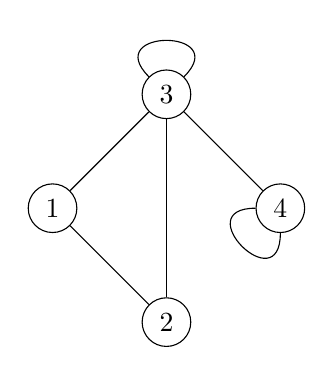
\begin{tikzpicture}[main/.style={draw,circle}]
							% Node plassering
							\node[main] (1) at (0,0) {1};
							\node[main] (2) [below right=of 1] {2};
							\node[main] (3) [above right=of 1] {3};
							\node[main] (4) [below right=of 3] {4};
							
							% Kant definisjon
							\graph {
								(3) -- (1) -- (2) -- (3) -- (4);
								};
								\draw (4) to [out=180, in=270, looseness=5] (4);
								\draw (3) to [out=45, in=135, looseness=5] (3);
							\end{tikzpicture}
						\end{center}
				\end{minipage}
			\end{onlyenv}
		\end{itemize}
	\end{frame}

	\begin{frame}{Kvantemynter}
		\begin{itemize}
			\item Hadamardmynten
			\begin{onlyenv}<1>
				\begin{itemize}
					\item $dim(\mathcal{H}_C)=2^n$
					\begin{align*}
						H_M = H^{\otimes n}
					\end{align*}
					\item $n = 2$
					\begin{align*}
						H_M = \frac{1}{2} \begin{pmatrix*}
							1 & 1 & 1 & 1 \\
							1 & -1 & 1 & -1 \\
							1 & 1 & -1 & -1 \\
							1 & -1 & -1 & 1
						\end{pmatrix*}
					\end{align*}
				\end{itemize}
			\end{onlyenv}
			\item Grovermynten
			\begin{onlyenv}<2>
				\begin{center}
					\begin{itemize}
						\item $dim(\mathcal{H}_C)=n$
						\begin{align*}
							d = \frac{1}{\sqrt{n}}\sum_{i=0}^{n-1}|i\rangle \\
							G_M = 2dd^* - I
						\end{align*}
						\item Anta $n = 4$
						\begin{align*}
							G_M = \frac{1}{2} \begin{pmatrix*}
								-1 & 1 & 1 & 1 \\
								1 & -1 & 1 & 1 \\
								1 & 1 & -1 & 1 \\
								1 & 1 & 1 & -1
							\end{pmatrix*}
						\end{align*}
					\end{itemize}
				\end{center}
			\end{onlyenv}
			\item Fouriermynten
			\begin{onlyenv}<3>
				\begin{itemize}
					\item $dim(\mathcal{H}_C)=n$
					\begin{align*}
						F_M = F_n
					\end{align*}
					\item La $\omega_{k,l}=e^{\frac{2\pi ikl}{n}}$
					\begin{align*}
						F_n = \frac{1}{\sqrt{n}} \begin{pmatrix*}
							\omega_{k,l}
						\end{pmatrix*}_{(k,l):\{0,...,n-1\}\times\{0,...,n-1\}}
					\end{align*}
				\end{itemize}
			\end{onlyenv}
		\end{itemize}
	\end{frame}

	\begin{frame}{Staggered model}
		\begin{itemize}
			\item Umyntet kvantevandring
			\item Bruker graftessellering for å definere $U$
			\item $\mathcal{H} = \mathbb{C}V$
			\begin{onlyenv}<1,4>
				\begin{flushleft}
					\begin{quantikz}
						\lstick{$\mathbb{C}V$} & \gate{U} & \qw
					\end{quantikz}
				\end{flushleft}
			\end{onlyenv}

			\begin{onlyenv}<2>
				\begin{center}
					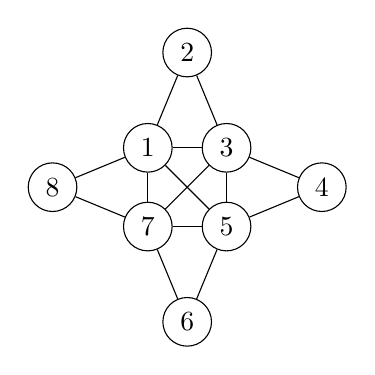
\begin{tikzpicture}[main/.style={draw,circle}, scale=1]
						%Nodene går her
						\node[main] (1) at (0,1) {1};
						\node[main] (2) at (0.5, 2.21) {2};
						\node[main] (3) at (1,1) {3};
						\node[main] (4) at (2.21, 0.5) {4};
						\node[main] (5) at (1,0) {5};
						\node[main] (6) at (0.5,-1.21) {6};
						\node[main] (7) at (0,0) {7};
						\node[main] (8) at (-1.21,0.5) {8};
	
						%Kantene defineres her
						\graph {
							(1) -- (2) -- (3) -- (1) -- (8) -- (7) -- (1) -- (5) -- (4) -- (3) -- (5) -- (6) -- (7) -- (5);
							(7) -- (3); 
						};
					\end{tikzpicture}
				\end{center}
			\end{onlyenv}
			\begin{onlyenv}<3>
				\begin{center}
					\begin{tcolorbox}
						\begin{minipage}{0.35\textwidth}
							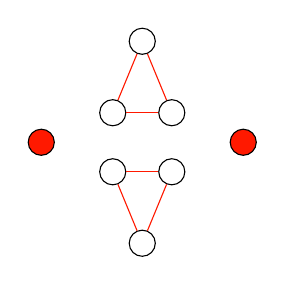
\begin{tikzpicture}[main/.style={draw,circle}, scale=0.75]
								%Nodene går her
								\node[main] (1) at (0,1) {};
								\node[main] (2) at (0.5, 2.21) {};
								\node[main] (3) at (1,1) {};
								\node[main, fill=red!80!orange] (4) at (2.21, 0.5) {};
								\node[main] (5) at (1,0) {};
								\node[main] (6) at (0.5,-1.21) {};
								\node[main] (7) at (0,0) {};
								\node[main, fill=red!80!orange] (8) at (-1.21,0.5) {};
			
								%Kantene defineres her
								\graph {
									(1) --[color=red!80!orange] (2) --[color=red!80!orange] (3) --[color=red!80!orange] (1);
									(5) --[color=red!80!orange] (6) --[color=red!80!orange]  (7) --[color=red!80!orange] (5);
									};
								
							\end{tikzpicture}
							{$\mathcal{T}_1$}
						\end{minipage}%
						\begin{minipage}{0.35\textwidth}
							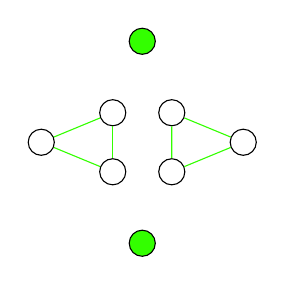
\begin{tikzpicture}[main/.style={draw,circle}, scale=0.75]
								%Nodene går her
								\node[main] (1) at (0,1) {};
								\node[main, fill=green!80!yellow] (2) at (0.5, 2.21) {};
								\node[main] (3) at (1,1) {};
								\node[main] (4) at (2.21, 0.5) {};
								\node[main] (5) at (1,0) {};
								\node[main, fill=green!80!yellow] (6) at (0.5,-1.21) {};
								\node[main] (7) at (0,0) {};
								\node[main] (8) at (-1.21,0.5) {};
			
								%Kantene defineres her
								\graph {
									(1) --[color=green!80!yellow] (7) --[color=green!80!yellow] (8) --[color=green!80!yellow] (1);
									(3) --[color=green!80!yellow] (4) --[color=green!80!yellow] (5) --[color=green!80!yellow] (3);
									};
								
							\end{tikzpicture}
							{$\mathcal{T}_2$}
						\end{minipage}%
						\begin{minipage}{0.35\textwidth}
							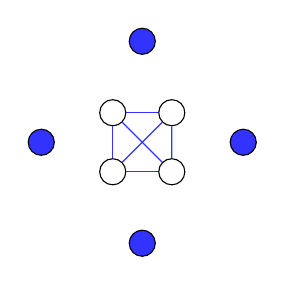
\begin{tikzpicture}[main/.style={draw,circle}, scale=0.75]
								%Nodene går her
								\node[main] (1) at (0,1) {};
								\node[main, fill = blue!80!white] (2) at (0.5, 2.21) {};
								\node[main] (3) at (1,1) {};
								\node[main, fill = blue!80!white] (4) at (2.21, 0.5) {};
								\node[main] (5) at (1,0) {};
								\node[main, fill = blue!80!white] (6) at (0.5,-1.21) {};
								\node[main] (7) at (0,0) {};
								\node[main, fill = blue!80!white] (8) at (-1.21,0.5) {};
			
								%Kantene defineres her
								\graph {
									(1) --[color=blue!80!white] (3) --[color=blue!80!white] (5) --[color=blue!80!white] (7) --[color=blue!80!white] (1) --[color=blue!80!white] (5);
									(7) --[color=blue!80!white] (3);
								};
								
							\end{tikzpicture}
							$\mathcal{T}_3$
						\end{minipage}
					\end{tcolorbox}
				\end{center}
			\end{onlyenv}

			\begin{onlyenv}<4>
				\item $U = \circ_{i}H_{\mathcal{T}_i}$
				\begin{align*}
					H_{\mathcal{T}_i} & =2\sum_{\alpha:\mathcal{T}_i}\alpha\alpha^* - I
				\end{align*}
			\end{onlyenv}
		\end{itemize}
	\end{frame}

	\begin{frame}{Grensepunktet og quasi-periodisitet}
		\begin{itemize}
			\item Hva skjer med kvantevandringen når $\lim_{k\rightarrow\infty}U^k(\psi_0)$?
			\begin{onlyenv}<2->
				\item $||U^{k+1}(\psi_0)-U^k(\psi_0)||$ er konstant for alle $k$
				\item Grensen konverger kun om $\psi_0$ er et fikspunkt for $U$
			\end{onlyenv}
			\begin{onlyenv}<3->
				\item Finnes det en $k$ slik at $U^k\psi_0=\psi_0$?
			\end{onlyenv}
			\begin{onlyenv}<4->
				\item Nei, dette gjelder ikke generelt
				\item Vi kan derimot finne en $k$ slik at $||U^k\psi_0-\psi_0||<\epsilon$ for en gitt $\epsilon > 0$
				\begin{align*}
					U = \begin{pmatrix*}
						e^{2\pi i\lambda_1} & 0 \\
						0 & e^{2\pi i\lambda_2}
					\end{pmatrix*}.
				\end{align*}
				\item Tilnærm $\lambda_i \approx \sfrac{a_i}{b_i}$, deretter sett $k=b_1b_2$
			\end{onlyenv}
		\end{itemize}
	\end{frame}

	\begin{frame}{Quantum Spatial Search}
		\begin{itemize}
			\item La $G=(V,E)$ og $f : V \rightarrow \{0,\ 1\}$ slik at nøyaktig 1 $v:V$ tilfredstiller $f(v)=1$
			\item Hvordan kan vi finne $v$? \\
			\begin{quantikz}
				\lstick{$\psi_0$} & \gate{O_{f,\pm}}\gategroup[wires = 1, steps = 2, style={rounded corners}]{S} & \gate{U} & \gate{S} & \qw \ldots & \gate{S} & \qw
			\end{quantikz}
			\item Kjøretiden $k$ er gitt ved å maksimere følgende funksjon
			\begin{align*}
				p(k) = |\langle v|S^k\psi_0\rangle|^2
			\end{align*}
			\item Grover er en optimal QSS algoritme
		\end{itemize}
	\end{frame}

\section{Implementasjon og tester}

	\begin{frame}{Kvantespråk}
		\begin{itemize}
			\item Qiskit
			\item Q\#
			\item Cirq
			\item Openql/Quantpy
			\item Quipper
			\item Quantum IO Monad
		\end{itemize}
	\end{frame}

	\begin{frame}{Position-coin simulering}
			\begin{onlyenv}<1>
				\includegraphics[scale=0.5]{Fig7Start0.png}
			\end{onlyenv}
			\begin{onlyenv}<2>
				\includegraphics[scale=0.5]{Fig7Hadamard.png}
			\end{onlyenv}
			\begin{onlyenv}<3>
				\includegraphics[scale=0.5]{Fig7GroverUniformMynt.png}
			\end{onlyenv}
	\end{frame}

	\begin{frame}{Arc simulering}
			\begin{onlyenv}<1>
				\includegraphics[scale = 0.5]{Fig9Start0.png}
			\end{onlyenv}
			\begin{onlyenv}<2>
				\includegraphics[scale = 0.5]{Fig9Hadamard.png}
			\end{onlyenv}
	\end{frame}

	\begin{frame}{Staggered simulering}
			\begin{onlyenv}<1>
				\includegraphics[scale = 0.5]{Fig10Start0.png}
			\end{onlyenv}
			\begin{onlyenv}<2>
				\includegraphics[scale = 0.5]{Fig10Hadamard.png}
			\end{onlyenv}
	\end{frame}

	\begin{frame}{QSS simulering}
			\begin{onlyenv}<1>
				\includegraphics[scale = 0.5]	{Fig10QSS.png}
			\end{onlyenv}
			\begin{onlyenv}<2>
				\includegraphics[scale = 0.5]	{Fig10QSSAmp.png}
			\end{onlyenv}
	\end{frame}

\section{Veien videre}

	\begin{frame}{Hvor kan man gå videre?}
		\begin{itemize}
			\item Szegedy vandring
			\item Kontinuerlige Kvantevandringer
			\item Flyt og elektriske nettverk
			\item Kriterier for optimalitet av kvantevandringer
			\item Kvantevandringer over grafer med mer struktur
			\item Hvordan bruke kvantevandringer til å løse problemer
		\end{itemize}
	\end{frame}

\end{document}